%%%%%%%%%%%%%%%%%%%%%%% file typeinst.tex %%%%%%%%%%%%%%%%%%%%%%%%%
%
% This is the LaTeX source for the instructions to authors using
% the LaTeX document class 'llncs.cls' for contributions to
% the Lecture Notes in Computer Sciences series.
% http://www.springer.com/lncs       Springer Heidelberg 2006/05/04
%
% It may be used as a template for your own input - copy it
% to a new file with a new name and use it as the basis
% for your article.
%
% NB: the document class 'llncs' has its own and detailed documentation, see
% ftp://ftp.springer.de/data/pubftp/pub/tex/latex/llncs/latex2e/llncsdoc.pdf
%
%%%%%%%%%%%%%%%%%%%%%%%%%%%%%%%%%%%%%%%%%%%%%%%%%%%%%%%%%%%%%%%%%%%


\documentclass[runningheads,a4paper]{llncs}

\usepackage{amssymb}
\setcounter{tocdepth}{3}
\usepackage{graphicx}

\usepackage{url}
\urldef{\mailsa}\path|{alfred.hofmann, ursula.barth, ingrid.haas, frank.holzwarth,|
\urldef{\mailsb}\path|anna.kramer, leonie.kunz, christine.reiss, nicole.sator,|
\urldef{\mailsc}\path|erika.siebert-cole, peter.strasser, lncs}@springer.com|    
\newcommand{\keywords}[1]{\par\addvspace\baselineskip
\noindent\keywordname\enspace\ignorespaces#1}

\begin{document}

\mainmatter  % start of an individual contribution

% first the title is needed
\title{Lecture Notes in Computer Science:\\Authors' Instructions
for the Preparation\\of Camera-Ready
Contributions\\to LNCS/LNAI/LNBI Proceedings}

% a short form should be given in case it is too long for the running head
\titlerunning{Lecture Notes in Computer Science: Authors' Instructions}

% the name(s) of the author(s) follow(s) next
%
% NB: Chinese authors should write their first names(s) in front of
% their surnames. This ensures that the names appear correctly in
% the running heads and the author index.
%
\author{Alfred Hofmann%
\thanks{Please note that the LNCS Editorial assumes that all authors have used
the western naming convention, with given names preceding surnames. This determines
the structure of the names in the running heads and the author index.}%
\and Ursula Barth\and Ingrid Haas\and Frank Holzwarth\and\\
Anna Kramer\and Leonie Kunz\and Christine Rei\ss\and\\
Nicole Sator\and Erika Siebert-Cole\and Peter Stra\ss er}
%
\authorrunning{Lecture Notes in Computer Science: Authors' Instructions}
% (feature abused for this document to repeat the title also on left hand pages)

% the affiliations are given next; don't give your e-mail address
% unless you accept that it will be published
\institute{Springer-Verlag, Computer Science Editorial,\\
Tiergartenstr. 17, 69121 Heidelberg, Germany\\
\mailsa\\
\mailsb\\
\mailsc\\
\url{http://www.springer.com/lncs}}

%
% NB: a more complex sample for affiliations and the mapping to the
% corresponding authors can be found in the file "llncs.dem"
% (search for the string "\mainmatter" where a contribution starts).
% "llncs.dem" accompanies the document class "llncs.cls".
%

\toctitle{Lecture Notes in Computer Science}
\tocauthor{Authors' Instructions}
\maketitle


\begin{abstract}

%Mention why convergence in PSO is a problem and why position
%diversity is essential to fix that problem.  

\end{abstract}


\section{Introduction}
\label{introduction}

Mention the hypothesis of the increase of position diversity and the random parameter.

\section{Related Work}
\label{related-work}

As has been demonstrated in practice, as
in \cite{garcia2014randomized}, \cite{gong2011distributed}, and
\cite{tanabe2013evaluation}, this approach obtains similar results to
an evolutionary algorithm with optimised parameters. % This probably
                                % should go to state of the art - JJ

\section{Preliminaries}
\label{preliminaries}

EvoSpace
Particle Swarm Optimisation (cognitive factor and social
factor). Formula.

\section{Proposed Method}
\label{proposed-method}

The proposed method is designed to accelerate the convergence of the
PSO algorithm. The hypothesis that was taken into consideration for this method is
that extending PSO to a parallel architecture should increase the
position diversity of the particles, and avoid premature convergence around a local
optimum and should yield better results because of this, as explained
by S. Cheng in \cite{cheng2013population}. Furthermore, each device in
the parallel architecture that is searching for a solution is configured with a
random set of parameters, as proposed by Y. Gong and
A. Fukunaga in \cite{gong2011distributed}. The intention of this approach is to
replace an optimization process of the parameters for a single instance of
an evolutionary algorithm, and, instead, use a number of instances with
different random parameters.  %Don't understand this - JJ

The PSO algorithm was adapted to integrate it with the EvoSpace
architecture \cite{garcia2015evospace}. EvoSpace enables different
instances of PSO to be working on a single population, taking random
samples of particles, and updating the positions of these particles
according to the randomly determined cognitive and social factors
(explained in Section \ref{preliminaries}) set to each instance of the
PSO algorithm. When a PSO instance requests a sample from the
population of particles, the best particle is also included in
the sample, i.e., the best particle considered is not the best in the
sample taken by the PSO instance, but the global best particle. This
ensures that all the PSO instances update the positions of its
samples' particles according to the global best.

All the PSO instances then proceed to update the sample particle
positions for a predetermined number of iterations. After the
iterations are completed, the sample is returned to the global
population in EvoSpace, and a new random sample is obtained by the PSO
instances that finished the evolutionary process and returned their
samples. This behaviour allows the PSO instances to update subsets of
particles of the population using different cognitive and social
factors.

As can be seen in Figure \ref{traditional-pso}, the particles in a
traditional PSO algorithm always move according to the best particle
(the red coloured particle, in this case) in each iteration, in terms
of the pre-established cognitive and
social factors. In contrast, one can see in Figure
\ref{distributed-pso} how the proposed method works. Each circled
group of particles have their positions updated in the plane according to the
social and cognitive factors of each PSO instance. In this case, each
circled group of particles represents a random sample of particles
taken from the population stored in EvoSpace. As was mentioned before,
this method should increase the diversity of the particles in the
population, and the randomized parameter setting should help particles
converge to a solution as fast as a PSO with dynamic adaptation of its
parameters.

\begin{figure}
  \centering
  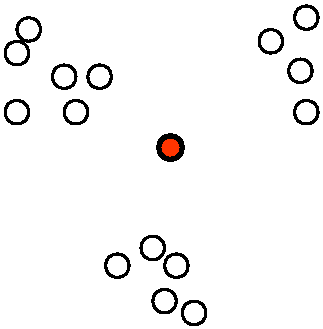
\includegraphics[height=4cm]{pdf/traditional-pso}
  \caption{}
  \label{traditional-pso}
\end{figure}

\begin{figure}
  \centering
  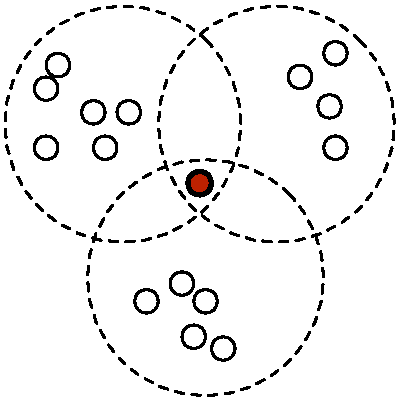
\includegraphics[height=4cm]{pdf/distributed-pso}
  \caption{}
  \label{distributed-pso}
\end{figure}

The diversity of the population of particles is calculated by using
the formula presented in (\ref{formula-diversity})

\begin{equation}
  \label{formula-diversity}
  D(P) = \frac{1}{|P|}\sum{i=1}^{|P|} \sqrt{}
\end{equation}

where blah blah blah %% finish formula first, and then explain

Lastly, the proposed method enables different physical devices to get
involved in the evolutionary process. A device can request a sample of
the particles and it updates their positions for a certain number of
generations. After finishing this process, the device returns the
updated sample to the EvoSpace server. This architecture allows the
physical devices to work asynchronously and in parallel.

\section{Experiments}
\label{experiments}

\section{Results}
\label{results}

\section{Conclusions}
\label{conclusions}

\section{Future Work}
\label{future-work}

\section{Acknowledgements}

We acknowledge support from 
Spanish Ministry of Economy and Competitiveness and European Regional
Development Fund (FEDER) under project EphemeCH
(TIN2014-56494-C4-3-P and  
from University of Granada, PROY-PP2015-06 (Plan Propio 2015 UGR)
\section{Cites}


\cite{garcia2015evospace}
\cite{garcia2014randomized}
\cite{merelo2012pool}
\cite{mussi2011gpu}
\cite{merelo2013designing}
\cite{merelo2008asynchronous}
\cite{morrison2001measurement}
\cite{roy2009distributed}
\cite{sherry2012flex}
\cite{tanabe2013evaluation}
\cite{de1990analysis}
\cite{melin2013optimal}
\cite{zadeh1988fuzzy}
\cite{zadeh1965fuzzy}
\cite{abdelbar2005fuzzy}
\cite{kenndy1995particle}
\cite{mcnabb2007parallel}
\cite{venter2006parallel}
\cite{koh2006parallel}
\cite{cheng2013population}
\cite{gong2011distributed}

\bibliographystyle{splncs03}
\bibliography{paper}

\end{document}
